%project-final-report.tex
\documentclass{article}
\usepackage[letterpaper, margin=1.2in]{geometry}
\usepackage{caption}
\usepackage{graphicx}
\usepackage{subcaption}
\usepackage{xcolor}
\usepackage{booktabs}
\usepackage{listings}
\usepackage{xparse}

\lstset{language=C,keywordstyle={\bfseries \color{blue}}}

\begin{document}

\title{A Benchmark of Linux System Calls}
\author{Jian Li \and Ding Yuan}
\maketitle

\section{Introduction}

The purpsoe of this paper is to evaluate the performance of Linux system calls of different kernel versions.


\section{Experiments}

We chose Linux kernel version 4.x (4.0 - 4.14) and 3.x (3.0 - 3.19) for our performance tests. The system calls tested are listed in Tablea \ref{tab:syscalls}.

\begin{table}
    \centering
    \begin{tabular}{clcclcclc}
        \toprule
        syscall \# & name & eax & syscall \# & name & eax & syscall \# & name & eax \\
        \midrule
        2 & fork & 0x02     &  15 & chhmod & 0x0f   &  41 & dup & 0x29 \\
        3 & read & 0x03     &  18 & stat & 0x12     &  42 & pipe & 0x2a \\
        4 & write & 0x04    &  20 & getpid & 0x14   &  43 & times & 0x2b \\
        5 & open & 0x05     &  25 & stime & 0x19    &  51 & acct & 0x33 \\
        6 & close & 0x06    &  27 & alarm & 0x1b    &  60 & umask & 0x3c \\
        9 & link & 0x09     &  28 & fstat & 0x1c    &  63 & dup2 & 0x3f \\
        10 & unlink & 0x0a  &  30 & utime & 0x1e    &  64 & getppid & 0x40 \\
        11 & execve & 0x0b  &  38 & rename & 0x26   &  65 & getpgrp & 0x41 \\
        13 & time & 0x0d    &  39 & mkdir & 0x27    & \\
        14 & mknod & 0x0e   &  40 & rmdir & 0x28    & \\
        \bottomrule
    \end{tabular}
    \caption{\label{tab:syscalls} System Calls for Performance Test}
\end{table}


\subsection{clock\_gettime vs. RDTSC}

\subsubsection{clock\_gettime}

A common way of measuring execution time is using C library function \lstinline{clock_gettime}.
Setting the argument \lstinline{clk_id} to \lstinline{CLOCK_REALTIME} will return the real clock time in nanoseconds precision,
which could be used to measure the execution of system calls.

The problem in using \lstinline{clock_gettime} is that \lstinline{clock_gettime} itself is a system call
and requires context switch, which could add significant overhead to the test result.
Although Linux kernel uses vsyscall and VDSOs (Virtual Dynamically linked Shared Objects) to minimize
the overhead by avoiding context switch, the latency is still too high when considering our purpose.

\subsubsection{RDTSC}

Intel ia64/x86 architecture provided RDTSC (Read Time-Stamp Counter) instruction\cite{rdtsc} for directly counting CPU cycles. 
RDTSC will read the cycle counter into eax and edx registers, which is a monotonic increasing number.
This can be used for performance test if compatibility is not a consideration.

The basic benchmark code with RDTSC is listed below.

\begin{verbatim}
        asm volatile("RDTSC\n\t"
                    "mov %%edx, %0\n\t"
                    "mov %%eax, %1\n\t" : "=r" (x0h), "=r" (x0l)::);
        test_function();
        asm volatile("RDTSC\n\t"
                    "mov %%edx, %0\n\t"
                    "mov %%eax, %1\n\t" : "=r" (x1h), "=r" (x1l)::);
        start = (((uint64_t)x0h << 32) | x0l);
        end = (((uint64_t)x1h << 32) | x1l);
        cycles = end - start;
\end{verbatim}

Since RDTSC can be called from user space directly, it could run much faster than \lstinline{clock_gettime}.
The problem in RDTSC is its hardware dependency, i.e. it is only available on Intel architecture.
In our experiments this is not a problem since we do not consider compatibility.

\subsubsection{Out-of-order execution}

Modern CPU is equipped with out-of-order execution feature.
This is used to optimize the penalties due to different instruction latencies,
however this will make our benchmark difficult, because there is no guarantee that
RDTSC will be executed exactly before and after the test code.

The solution includes two extra instruction. First, the CPUID instruction will be called before RDTSC
instruction. CPUID can be executed at any privilege level and will force the CPU to serialize any instructions
before CPUID. In this way the CPUID and the following RDTSC can be guaranteed to be run before the test code.

However for the RDTSC call after the test function,
it is still possible for the instructions after RDTSC to be executed before RDTSC but after CPUID.
To solve this, RDTSCP instruction can be used insted of CPUID and RDTSC.
RDTSCP will read both cycle counter and CPU id, which is essentially an "atomic" operation
to ensure serialized instructions.

\subsubsection{Exclusive CPU ownership}

It is common to disble preemption(\lstinline{preempt_disable()}) and hard interrupts(\lstinline{raw_local_irq_save()})
to guarantee the exclusive CPU ownership when measuring CPU cycles. However in our case, these two functions
are only available in kernel mode, which is not reasonable when behchmarking system calls.
Therefore we will not use these functions.

\subsection{Environment}

The computer we used to run the benchmark test has an Intel Core i3-4300 CPU with 16GB memory. The CPU frequency is 3491.851MHz. The Linux OS is Ubuntu 16.04.

\subsubsection{Linux Setup}

The benchmarking is required to be repeated on multiple Linux kernels.
To minimize the overhead of compiling Linux kernels,
we decided to install pre-built kernel from Ubuntu kernel PPA\cite{kernelppa}. 

The kernel versions varies from 3.2 to 4.14. We were unable to test 3.1 and older kernels since they could not boot under Ubuntu 16.04.

In order to automate the benchmarking, a python script is used to automatically switch the default kernel by changing the grub config.
The linux OS as been changed so that root user will automatically login and execute the benchmark scripts after boot.


\section{Benchmark}

The basic benchmark is to fetch the cycle counter before and after the target system call so that the consumed cycles can be calculated.
However some system calls require special operations.

\subsection{fork}

\lstinline{fork} will create an identical process of the caller so that regular operation cannot be used.
In order to measure this, both parent and child process will fetch the cycle counter after \lstinline{fork()} is called.
Shared memory is used to pass the child counter back to the parent counter.
A pipe is created between the parent and child processes and the parent process writes into the pipe to force
the OS scheduler to switch to the child process. Then the parent process will wait for the child process.
After that, the parent process will compare the cycle counters from both parent and child processes
and use the greater one as the final result.

\subsection{unlink}

In Linux, \lstinline{unlink()} system call will decrease the (hard) link counter and remove the file if the last link is removed.
Therefore it is necessary to measure \lstinline{unlink()} in two cases: removing the last link, and remove the non-last link.
Our experiment results show that different cycles are required in these two cases, and the difference is the cycles required for removing the file itself.


\subsection{Benchmark Results}

Due to limited space we only show part of the benchmark result here. Full result can be found at the project website\footnote{https://github.com/charlee/linux-prof}.
The average cycles cost by system calls of major Linux kernel version are listed in Table \ref{tab:mean}.


\begin{table}
    \centering
    \begin{tabular}{clrrrrr}
        \toprule
        eax & syscall & 3.2.96 & 3.10.108 & 3.19.8 & 4.4.0 & 4.14.0 \\
        \midrule
        02 & fork & 332512 & 88102 & 86261 & 93924 & 184170 \\
        03 & read & 10189 & 3603 & 2694 & 2796 & 4811 \\
        04 & write & 62045 & 16674 & 17113 & 16600 & 32780 \\
        05 & open & 100012 & 27445 & 30248 & 27760 & 49898 \\
        06 & close & 7924 & 4107 & 2668 & 2373 & 3916 \\
        09 & link & 43976 & 13146 & 9603 & 8812 & 16122 \\
        0a & unlink & 34974 & 10104 & 8838 & 7958 & 14561 \\
        0b & execve & 33513 & 9751 & 11403 & 11223 & 18058 \\
        0d & time & 6373 & 1532 & 1484 & 1462 & 8778 \\
        0e & mknod & 92496 & 25768 & 28424 & 25766 & 45868 \\
        0f & chmod & 37023 & 10900 & 7334 & 7505 & 13152 \\
        12 & stat & 19895 & 6797 & 2953 & 3068 & 5668 \\
        14 & getpid & 4274 & 1889 & 995 & 1025 & 1841 \\
        19 & stime & 17381 & 79772 & 56543 & 87464 & 95605 \\
        1b & alarm & 21137 & 6488 & 7607 & 7782 & 12416 \\
        1c & fstat & 7274 & 5386 & 1775 & 1789 & 2531 \\
        1e & utime & 34401 & 10126 & 6265 & 6370 & 11371 \\
        26 & rename & 78948 & 20912 & 19564 & 17162 & 30875 \\
        27 & mkdir & 183147 & 45946 & 50873 & 45946 & 85106 \\
        28 & rmdir & 147876 & 39826 & 38157 & 31147 & 59144 \\
        29 & dup & 6033 & 2621 & 1542 & 1483 & 2649 \\
        2a & pipe & 7020 & 9005 & 10604 & 10995 & 10873 \\
        2b & times & 17309 & 5744 & 7581 & 7341 & 11993 \\
        2c & acct & 30622 & 8507 & 9630 & 10846 & 17090 \\
        3c & umask & 12934 & 4827 & 5967 & 6193 & 9510 \\
        3f & dup2 & 5923 & 2662 & 1505 & 1455 & 2624 \\
        40 & getppid & 13194 & 4961 & 6007 & 6111 & 9435 \\
        41 & getpgrp & 13115 & 5082 & 6088 & 6251 & 9509 \\
        \bottomrule
    \end{tabular}
    \caption{\label{tab:mean} Average Cycles for System Calls in Major Kernel Versions}
\end{table}


For each system calls, the average cycles required keep almost unchanged for most of the system calls we measured.
However the cycles required dropped significantly when kernel version is upgraded from 3.9 to 3.10.
For example, \lstinline{unlink} requires approximately 35000 cycles in kernel version 3.9, but
only requires approximately 10000 cycles in 3.10. We assume that there was a major performance improvement in kernel 3.10,
however the detail will require further investigation.

\begin{figure}[h!]
    \centering
    \begin{subfigure}[b]{0.3\textwidth}
        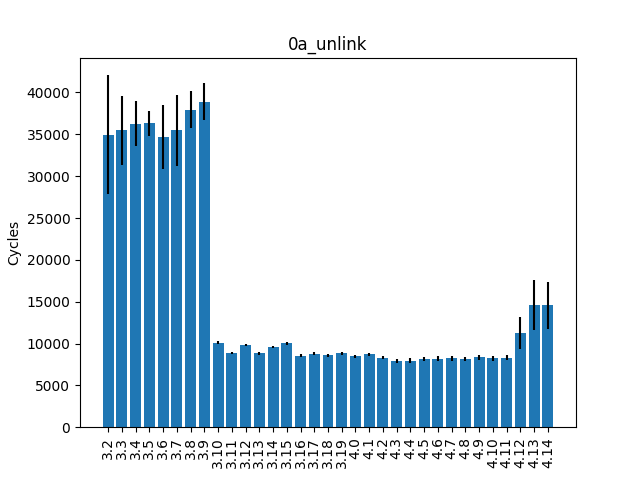
\includegraphics[width=\textwidth]{../report/0a_unlink.png}
        \caption{unlink}
    \end{subfigure}
    \begin{subfigure}[b]{0.3\textwidth}
        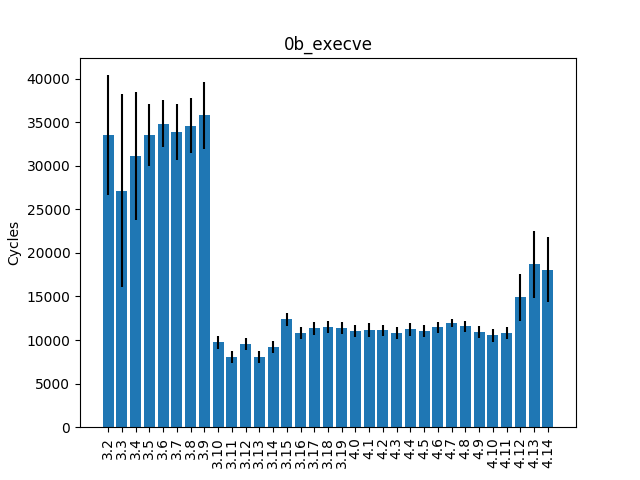
\includegraphics[width=\textwidth]{../report/0b_execve.png}
        \caption{execve}
    \end{subfigure}
    \begin{subfigure}[b]{0.3\textwidth}
        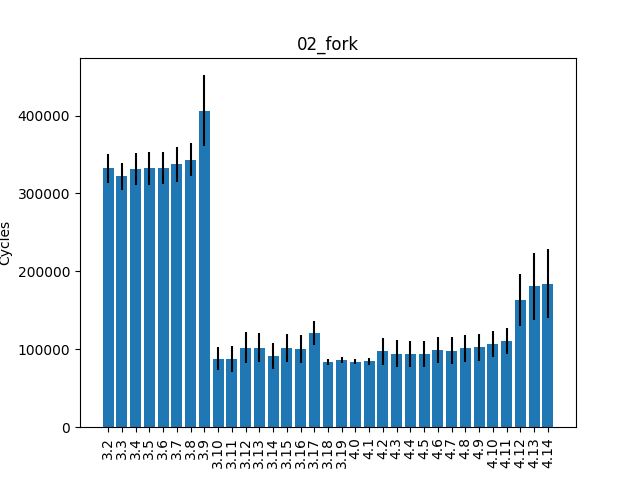
\includegraphics[width=\textwidth]{../report/02_fork.png}
        \caption{fork}
    \end{subfigure}

    \begin{subfigure}[b]{0.3\textwidth}
        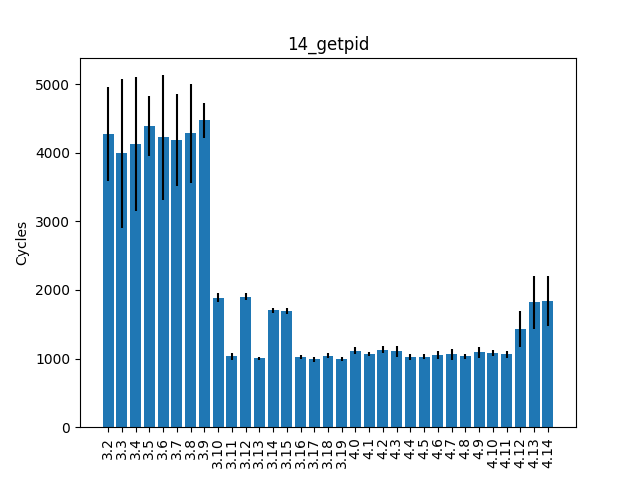
\includegraphics[width=\textwidth]{../report/14_getpid.png}
        \caption{getpid}
    \end{subfigure}
    \begin{subfigure}[b]{0.3\textwidth}
        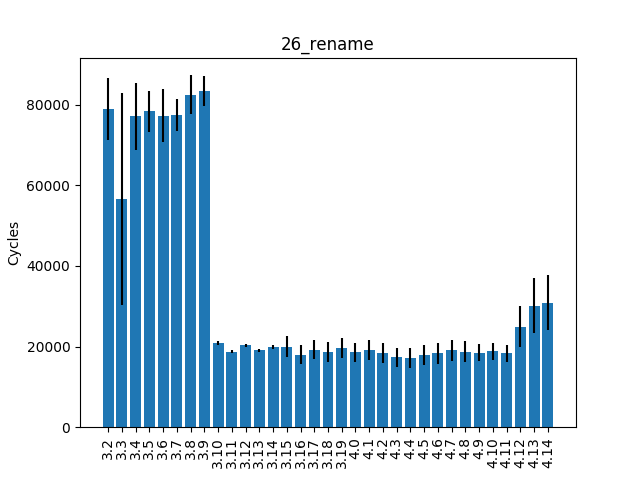
\includegraphics[width=\textwidth]{../report/26_rename.png}
        \caption{rename}
    \end{subfigure}
    \begin{subfigure}[b]{0.3\textwidth}
        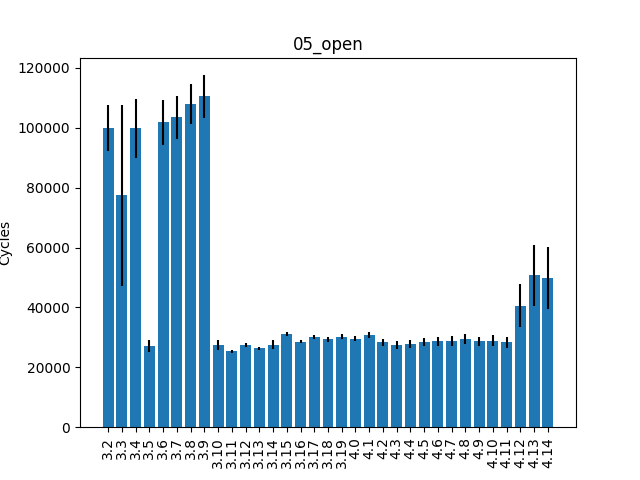
\includegraphics[width=\textwidth]{../report/05_open.png}
        \caption{open}
    \end{subfigure}
    \caption{Cycles for some System Calls}
    \label{fig:cycles}
\end{figure}


\section{Appendix}

\subsection{Linux settings}

To boot Ubuntu into text mode, use:

\begin{verbatim}
    sudo systemctl enable multi-user.target
    sudo systemctl set-default multi-user.target
\end{verbatim}

To run grub in text mode, change /etc/default/grub as:

\begin{verbatim}
    GRUB_CMDLINE_LINUX_DEFAULT="text nomodeset"
\end{verbatim}

To login as root user, edit /lib/systemd/system/getty@:

\begin{verbatim}
    ExecStart=-/sbin/agetty -a <USERNAME> --noclear %I $TERM
\end{verbatim}


\begin{thebibliography}{9}
    \raggedright
    \bibitem{kernelppa}
    \emph{Ubuntu Kernel PPA},
    http://kernel.ubuntu.com/~kernel-ppa/mainline/

    \bibitem{rdtsc}
    \emph{How to Benchmark Code Executions Times on Intel IA-32 and IA-64 Instruction Set Architectures},
    Intel Corporation,
    https://www.intel.com/content/dam/www/public/us/en/documents/white-papers/ia-32-ia-64-benchmark-code-execution-paper.pdf
\end{thebibliography}


\end{document}

